\documentclass[11pt]{article}
\usepackage{amsfonts}
\usepackage{hyperref}
\usepackage{graphicx,subfigure}
\usepackage{epsfig}
\usepackage{hyperref}
\usepackage{amsmath}
\usepackage{amssymb}
\usepackage{algorithm}
\usepackage{algorithmic}
\usepackage{url}
\usepackage{enumerate}
\usepackage{amsfonts}
\usepackage{boxedminipage}
\usepackage{xcolor}
 \usepackage{framed}  
\usepackage{rotating}
\usepackage{array}
\usepackage{multirow}
\usepackage{color}
\usepackage{tikz}
\usepackage{mathabx}
\usepackage{tabularx,ragged2e,booktabs,caption}
\usepackage{enumitem}
\newcommand{\overbar}[1]{\mkern 1.5mu\overline{\mkern-1.5mu#1\mkern-1.5mu}\mkern 1.5mu}

\oddsidemargin=0.15in
\evensidemargin=0.15in
\topmargin=-.5in
\textheight=9in
\textwidth=6.25in



\DeclareGraphicsExtensions{.gif, .ps, .eps, .png}
\DeclareGraphicsRule{.gif}{png}{}{`convert #1 'png:-'}

\newcommand{\inprod}[2]{\left\langle #1,#2\right\rangle}
\newcommand{\norm}[1]{\left\| #1\right\|}
\newcommand{\pmat}[1]{\begin{pmatrix} #1\end{pmatrix}}
\newcommand{\cB}{\mathcal{B}}
%\newcommand{\cD}{\mathcal{D}}
%\newcommand{\bE}{\mathbb{E}\,}
\newcommand{\bN}{\mathbb{N}\,}

\title{{\large{Introduction to Machine Learning (67577)}}\\
\vphantom{}Lecture 1 \\
Introduction to Introduction to ML: Probability}

\date{February 2019}

\usepackage{graphicx,subfigure}
% As of 2010, we use the hyperref package to produce hyperlinks in the
% resulting PDF.  If this breaks your system, please commend out the
% following usepackage line and replace \usepackage{icml2011} with
% \usepackage[nohyperref]{icml2011} above.
\usepackage{hyperref}

% \usepackage{icml2011} 

\usepackage{amsmath}
\usepackage{amssymb}

\usepackage{algorithm}
\usepackage{algorithmic}
\algsetup{indent=2em}


%% \usepackage{rotating}
%% \usepackage{array}
%% \usepackage{multirow}
%% \usepackage{color}

%% \usepackage{tikz}

\usepackage{url}

\newtheorem{definition}{Definition}
\newtheorem{lemma}{Lemma}
\newtheorem{corollary}{Corollary}
\newtheorem{theorem}{Theorem}
\newtheorem{proposition}{Proposition}
\newtheorem{assumption}{Assumption}
\newtheorem{example}{Example}
\newtheorem{remark}{Remark}
\newtheorem{claim}{Claim}
\newtheorem{exercise}{Exercise}
\newtheorem{discussion}{Discussion}


\newcommand{\gb}[1]{{\boldsymbol{#1}}}
\newcommand{\valpha}{\gb{\alpha}}
\newcommand{\vmu}{\gb{\mu}}
\newcommand{\vnu}{\gb{\nu}}
\newcommand{\vxi}{\gb{\xi}}
\newcommand{\vtheta}{\gb{\theta}}
\newcommand{\vrho}{\gb{\rho}}
\newcommand{\vbeta}{\gb{\beta}}
\newcommand{\vtau}{\gb{\tau}}
\newcommand{\vbalpha}{\gb{\alpha^\star}}
\newcommand{\vbbeta}{\gb{\beta^\star}}
\newcommand{\vtalpha}{\gb{\tilde{\alpha}}}
\newcommand{\vlambda}{\gb{\lambda}}
\newcommand{\slambda}{\bar{\vlambda}}
\newcommand{\stheta}{\bar{\vtheta}}
\newcommand{\vphi}{\gb{\phi}}
\newcommand{\vsigma}{\gb{\sigma}}

\newcommand{\x}{{\mathbf x}}
\newcommand{\y}{{\mathbf y}}
\newcommand{\z}{{\mathbf z}}
\newcommand{\w}{{\mathbf w}}
\newcommand{\bw}{\bar{\w}}
\newcommand{\bF}{\bar{F}}
\renewcommand{\v}{{\mathbf v}}
\renewcommand{\u}{{\mathbf u}}
\newcommand{\e}{{\mathbf e}}
\newcommand{\bsig}{{\mathbf \sigma}}
\newcommand{\rE}{{\mathbf E}}
\newcommand{\sgn}{{\mathrm{sgn}}}
\newcommand{\cF}{{\cal F}}
\newcommand{\pr}{\mathbb{P}}
\newcommand{\rV}{{\mathrm {Var}}}
\newcommand{\tr}{{\mathrm{tr}}}
\newcommand{\trans}{\dagger}
\newcommand{\diag}{{\mathrm{diag}}}
\newcommand{\lspan}{{\mathrm{span}}}
\renewcommand{\r}{{\mathbf{r}}}
\newcommand{\tL}{\tilde{L}}
\newcommand{\hL}{\hat{L}}

\newcommand{\cD}{\mathcal{D}}
\newcommand{\bE}{\mathbb{E}\,}


\newcommand{\BlackBox}{\rule{1.5ex}{1.5ex}}  
\newenvironment{proof}{\par\noindent{\bf Proof\ }}{\hfill\BlackBox\\[2mm]}

\newcommand{\reals}{\mathbb{R}}
\newcommand{\Y}{\mathcal{Y}}
\newcommand{\X}{\mathcal{X}}
\renewcommand{\H}{\mathcal{H}}
\newcommand{\E}{\mathbb{E}}
\newcommand{\D}{\mathcal{D}}
\newcommand{\V}{\mathcal{V}}
\newcommand{\U}{\mathcal{U}}
\newcommand{\F}{\mathcal{F}}
\newcommand{\inner}[1]{\langle #1 \rangle}
\newcommand{\half}{\frac{1}{2}}
\newcommand{\thalf}{\tfrac{1}{2}}
\newcommand{\eqdef}{\stackrel{\mathrm{def}}{=}}
\newcommand{\err}{\mathrm{err}}
\newcommand{\opt}{\mathrm{opt}}
\newcommand{\herr}{\widehat{\err}}
\newcommand{\hopt}{\hat{\opt}}
\newcommand{\eopt}{\epsilon_{\mathrm{opt}}}
\newcommand{\eapp}{\epsilon_{\mathrm{app}}}
\newcommand{\eest}{\epsilon_{\mathrm{est}}}
\newcommand{\halg}{\tilde{h}}
\newcommand{\empf}{\hat{F}_{\lambda}}
\newcommand{\T}{\mathrm{time}}
\newcommand{\erf}{\mathrm{erf}}
\newcommand{\sig}{\mathrm{sig}}
\newcommand{\poly}{\mathrm{poly}}

\newcommand{\rank}{\mathrm{rank}}
\newcommand{\supp}{\mathrm{supp}}
\newcommand{\spn}{\mathrm{span}}
\newcommand{\image}{\mathrm{image}}


\DeclareMathOperator*{\argmin}{argmin} % Declares argmin and ensures super and subscripts are located nicely above/below such as in \min
\DeclareMathOperator*{\argmax}{argmax} % Declares argmin and ensures super and subscripts are located nicely above/below such as in \min
\DeclareMathOperator*{\prob}{\mathbb{P}} 

\renewcommand{\eqref}[1]{Equation~(\ref{#1})}
\newcommand{\figref}[1]{Figure~\ref{#1}}
\newcommand{\secref}[1]{Section~\ref{#1}}
\newcommand{\thmref}[1]{Theorem~\ref{#1}}
\newcommand{\lemref}[1]{Lemma~\ref{#1}}
\newcommand{\defref}[1]{Definition~\ref{#1}}
\newcommand{\corref}[1]{Corollary~\ref{#1}}

%\newcommand{\comment}[1]{\textcolor{red}{\textbf{#1}}}
\newcommand{\mathcomment}[1]{\color{red}{\textbf{#1}}}

\newcommand{\indct}[1]{\boldsymbol{1}\!\left[ #1 \right]}

\newcommand{\blambda}{\bar{\lambda}}
\newcommand{\bA}{\bar{A}}
\newcommand{\bI}{\bar{I}}

\newcommand{\vect}{\mathrm{vec}}


\newcommand{\coursename}{Introduction to Machine Learning (67577)}

\newcommand{\handout}[5]{
%   \renewcommand{\thepage}{#1-\arabic{page}}
   \noindent
   \begin{center}
   \framebox{
      \vbox{
    \hbox to 5.78in { {\bf \coursename}
         \hfill #2 }
       \vspace{4mm}
       \hbox to 5.78in { {\Large \hfill #5  \hfill} }
       \vspace{2mm}
       \hbox to 5.78in { {\it #3 \hfill #4} }
      }
   }
   \end{center}
   \vspace*{4mm}
}

\newcommand{\notes}[5]{
%   \renewcommand{\thepage}{#1-\arabic{page}}
   \noindent
   \begin{center}
    \hbox to 5.78in { {\bf \coursename}  \hfill #2}
       \vspace{14mm}
       \hbox to 5.78in { {\Large \hfill #5  \hfill} }
   \end{center}
   \vspace*{4mm}
}

% Lecture notes:
\newcommand{\lecture}[5]{\handout{#1}{#3}{Lecturer:
#4}{Scribe: #5}{Lecture #1: #2}}

\newcommand{\recitation}[5]{\handout{#1}{#3}{#4}{ #5}{Recitation #1: #2}}

% Exam:
\newcommand{\exam}[1]{\handout{#1}{}{}{}{Exam}}
\newcommand{\homeexam}[2]{\handout{#1}{}{}{Due:
#2}{Home Exam}}
\newcommand{\examanswer}[1]{\handout{X}{}{by: #1}{}{Exam - Answers}}

% New exercise
\newcommand{\problemset}[2]{\handout{#1}{}{}{Due:
#2}{Problem Set #1}}

% School solution
\newcommand{\solution}[2]{\handout{#1}{}{}{Written by: #2}{Problem Set #1 - Solution}}

% Submitted solution
\newcommand{\exanswer}[2]{\handout{#1}{}{by: #2}{}{Problem Set #1 - Answers}}

\begin{document}
\maketitle

\tableofcontents
\pagebreak

\section{Probability: Recap}
\subsection{Probability Space}
\footnote{This section based on lecture notes by Michal Moshkovitz and Alon Gonen} Our intuitive notion of probability is related to uncertainty we have about events in the world, for example - will it rain tomorrow? How much will I get in the final exam? Although we cannot predict with certainty the answers to these questions, we usually know what is the set of all possible outcomes. This gives us the first ingredient in any \emph{probability space}.
\begin{definition}
A \textit{sample space} $\Omega$ is a set that contains all possible outcomes.

$\omega\in\Omega$ denotes a single outcome.
\end{definition}
Examples:
\begin{itemize}
\item Coin toss: $\Omega=\left\{ H,T\right\} $
\item Toss a coin until heads comes up: $\Omega=\left\{ T^{n-1}H:n\in\mathbb{N}\right\} $
\item Rolling two (distinguishable) dice: $\Omega=\left\{ 1,\dots,6\right\} ^{2}$
What will be the sample space if the dice are indistinguishable? $\Omega=\left\{ \left(i,j\right):1\le i\le j\le6\right\} $
\item Waiting time at the post office: $\Omega=[0,\infty)$
\end{itemize}
Suppose someone threw a dice, and told us that the result is an even number. This result is not an element in $\Omega$, but it tells us that the outcome is an element in the subset $\left\{ 2,4,6\right\} $.
\begin{definition}
An \textit{event} $A$ is any subset of possible outcomes, $A\subseteq\Omega$.
\end{definition}
Quick reminder:
\begin{itemize}
\item $A^{c}$ (or sometimes $\overline{A}$) denotes the \textit{complement} of $A$, $A^{c}=\Omega\backslash A$ . In other words, $A^{c}$ is the event that $A$ did not occur. 
\item We say that $A$ and $B$ are \textit{disjoint} \textit{events} if $A\cap B=\emptyset$.
\item $\Omega$ and $\emptyset$ are also events. If $A$ and $B$ are two events, then $A\cup B$ is also an event, and so is $A\cap B$. 
\end{itemize}

Intuitively, a probability function assigns to an event a number which quantifies our knowledge or belief about the possibility of observing any outcome in that event. 


%\subsubsection*{Discrete models }
\begin{definition}
A probability space is a tuple \footnote{For our needs this simple and intuitive definition is suffice, though, richer definitions exist.} $(\Omega, \cD)$ where $\Omega$ is a \emph{sample space} and $\cD:2^{\Omega}\rightarrow\reals$ is a probability function such that 
\begin{enumerate}
\item $\cD(\Omega)=1$
\item for all $\omega\in\Omega,;\cD(\omega)\in[0,1]$
\item for all $A,B\subseteq\Omega$ such that $A\cap B=\emptyset,$ we have $\cD(A \cup B)=\cD(A)+\cD(B).$
\end{enumerate}
\end{definition} 
%\begin{exercise} Find he probability space that corresponds to a fair coin toss.
%\end{exercise}
%Solution: $\Omega=\{H,T\},\Pr(H)=\Pr(T)=0.5$
\begin{example}
Suppose we throw two fair dice, $\Omega=\left\{ 1,\dots,6\right\} ^{2}$ and $\cD\left(\left(i,j\right)\right)=\frac{1}{36}$
\end{example}

\begin{exercise}
For all $A,B\subseteq\Omega$: $\cD(A\cup B)=\cD(A)+\cD(B)-\cD(A\cap B)$
\end{exercise}
Solution:\\
$A\cup B=(A\setminus B)\cup(B\setminus A)\cup(A\cap B)\; ,A=(A\setminus B)\cup(A\cap B)$ and $B=(B\setminus A)\cup(A\cap B).$
$$\cD(A\cup B)=\cD(A\setminus B)+\cD(B\setminus A)+\cD(A\cap B)=\cD(A)-\cD(A\cap B)+\cD(B)-\cD(A\cap B)+\cD(A\cap B)$$ 

\begin{definition}
$A,B\subseteq\Omega$ are called \emph{independent} if $$\cD(A\cap B) =\cD(A)\cdot\cD(B).$$
\end{definition}

\begin{exercise}
If $A$ and $B$ are independent then $A$ and $B^c$ are also independent. 
\end{exercise}
Solution: $\cD(A)=\cD(A\cap B)+\cD(A\cap B^c)\Rightarrow\cD(A\cap B^c)=\cD(A)(1-\cD(B))=\cD(A)\cdot\cD(B^c).$\\


\begin{lemma}  \label{lem:unionBound}  \textbf{(The union bound)} Let
$(\Omega, \cD)$ be a probability space. The probability function is \emph{sub-additive}, i.e., for any sequence $(A_k)$ of events,
\[
\cD(\cup_{k=1}^\infty A_k) \le \sum_{k=1} ^\infty \cD(A_k)
\]
\end{lemma}
\begin{proof}
Let $B_1=A_1$. For each $k \in \{2,3,\ldots\}$, let $B_k = A_k
\setminus \cup_{i=1}^{k-1} A_i$. Note that the $B_1...B_k$ are disjoint, and
$\cup_{i=1}^k A_i=\cup_{i=1}^k B_i$. Also, since $B_k\subseteq A_k$, $\cD(B_k) \le \cD(A_k)$ for every $k \in \bN$. It follows by the countable additivity of $\cD$ that
\[
\cD(\cup_{k=1}^\infty A_k) = \cD(\cup_{k=1}^\infty B_k) = \sum_{k=1}
^\infty \cD(B_k) \le \sum_{k=1}
^\infty \cD(A_k)~. 
\]
\end{proof} 




\subsection{Random Variables}

So far we have asked questions like: does an event happen or not and what is the probability of the event. What if we want to know "how much." For example, we get a dollar if a a coin flip turns head. How many dollars we have after 3 rounds? In this case $\Omega=\{HHH,HHT,HTH,THH,THT,TTH,TTT\}$ and we can define a function that indicate the many we earn: $M(HHH)=3,M(HHT)=2.$ The function $M$ is called \emph{random variable.}
\begin{definition}
Given a probability space $\left(\Omega,\cD\right)$, a \textit{real-valued
random variable} is a function $X:\Omega\rightarrow\mathbb{R}$.

\end{definition}
\begin{remark}
Any function $g\left(X\right)$ of a random variable is also a random
variable (for instance $X^{2}$, $sign\left(X\right)$, etc.).
\end{remark}
For a discrete $\Omega$ we define the \textbf{\textit{probability
mass function}} of $X$ (a \textit{discrete RV}) as 
\[
\cD\left(\left\{ X=x\right\} \right)=\sum_{\omega:X\left(\omega\right)=x}\cD\left(\omega\right)
\]


Instead of writing $\cD\left(\left\{ X=x\right\} \right)$ we usually
write $\cD\left(x\right)$.

\begin{example}
A fair coin is tossed twice. The probability space  is $\Omega=\left\{ T,H\right\} ^{2}$
and $\cD\left(\omega\right)=\frac{1}{4}$. Let $X$ be the number of
times heads came up. In this case we have $\mathcal{X}=\left\{ 0,1,2\right\} $
and
\[
\cD\left(x\right)=\begin{cases}
\frac{1}{4} & x=0,2\\
\frac{1}{2} & x=1\\
0 & \mbox{else}
\end{cases}
\]

\end{example}
For a continuous $\Omega$ - we say that $X$ is a \textit{continuous
RV} if we can write for every $D\subset\mathbb{R}$ 
\[
\cD\left(X\in D\right)=\int_{D}f\left(x\right)dx
\]


In particular, this means we can write for every $\left[a,b\right]\subset\mathbb{R}$
\[
\cD\left(X\in\left[a,b\right]\right)=\int_{a}^{b}f\left(x\right)dx
\]


Note, that for any $a\in\mathbb{R}$ $\cD\left(X=a\right)=\int_{a}^{a}f\left(x\right)dx=0$.

The function $f$ is called the \textbf{\textit{probability density
function }}\textbf{(PDF)} of $X$. Note that - 
\begin{itemize}
\item $f\left(x\right)\ge0$
\item $\int_{-\infty}^{\infty}f\left(x\right)dx=1$ 
\item $f\left(x\right)$ is not a probability, and it could be that $f\left(x\right)>1$.\\
\end{itemize}

\subsection{Mean and Variance}
\begin{definition}
The \textbf{\textit{expected value}} of a random variable
$X$ is
\[
\bE\left[X\right]=\sum_{x\in\mathcal{X}}x\prob\left(x\right)\qquad\mbox{or}\qquad \bE\left[X\right]=\int_{-\infty}^{\infty}xf\left(x\right)dx
\]

\end{definition}
Properties:
\begin{itemize}
\item $\bE\left[g\left(X\right)\right]=\sum g\left(x\right)\cD\left(x\right)$,
\item $E\left[c\right]=c$
\item Linear: $\bE\left[aX+Y\right]=a\bE\left[X\right]+\bE\left[Y\right]$
\item If $X$ and $Y$ are independent then $\bE\left[XY\right]=\bE\left[X\right]\bE\left[Y\right]$
(explanation: $\bE[XY]=\sum\cD(X=x,Y=y)x\cdot y = \sum_{x,y}\cD(x)\cD(y)xy=\bE[X]\bE[Y]$)
\end{itemize}

\begin{definition}
Let $X$ be a RV with $ֿ\bE\left[X\right]=\mu$, then the \textbf{\textit{variance}}
of $X$ is 
\[
V\left(X\right)=\bE\left[\left(X-\mu\right)^{2}\right]
\]
The \textbf{\textit{standard deviation}} is defined as $\sigma=\sqrt{V\left(X\right)}$.
\end{definition}
Properties of the variance:
\begin{itemize}
\item $V(X)\geq0$ , ~$V(X)=0\,\iff\,X$ is a constant.
\item $V\left(X\right)=\bE\left[X^{2}\right]-\bE^{2}\left[X\right]$
\item $V(aX+b)=a^{2}V(X)$
\item $V(X+Y)=\bE\left[\left(X+Y-\bE(X)-\bE(Y)\right)^{2}\right]=V(X)+V(Y)+2\overbrace{\bE\left[\left(X-\bE[X]\right)\left(Y-\bE[Y]\right)\right]}^{Cov\left(X,Y\right)}$
\item If $X_{1},\dots,X_{n}$ are independent then $V\left(\sum X_{i}\right)=\sum V\left(X_{i}\right)$\end{itemize}

\begin{exercise}
Let $Z$ be a Bernoulli random variable. Calculate $Var[Z].$ 
\end{exercise}
Solution: $Var[Z]=E[Z^2]-E^2[Z]=p-p^2=p(1-p).$

\begin{definition}
The \textbf{\textit{covariance}} of $X$ and $Y$ is
\end{definition}
\[
Cov(X,Y)=\bE\left[\left(X-\bE[X]\right)\left(Y-\bE[Y]\right)\right]=\bE\left[XY\right]-\bE[X]\bE[Y]
\]


Properties:
\begin{itemize}
\item $Cov(X,Y)=Cov(Y,X)$
\item $Cov(aX+b,cY+d)=acCov(X,Y)$
\item $Cov(X,X)=V(X)$
\end{itemize}
%We say that $X$ and $Y$ are \textbf{\emph{uncorrelated}}\emph{ }\textit{\emph{if $Cov\left(X,Y\right)=0$.}}
%\begin{remark}
%If $X$ and $Y$ are uncorrelated it does not imply that they are independent.\end{remark}

\begin{example}
Find the mean and variance of $X\sim U\left(\left[a,b\right]\right),$ where $U[a,b]$ is the uniform distribution on $[a,b].$
\begin{eqnarray*}
\bE\left[X\right] & = & \frac{1}{b-a}\int_{a}^{b}xdx=\frac{1}{2\left(b-a\right)}\left(b^{2}-a^{2}\right)=\frac{b+a}{2}\\
\bE\left[X^{2}\right] & = & \frac{1}{b-a}\int_{a}^{b}x^{2}dx=\frac{1}{3\left(b-a\right)}\left(b^{3}-a^{3}\right)=\frac{b^{2}+ab+a^{2}}{3}\\
V\left(X\right) & = & \frac{b^{2}+ab+a^{2}}{3}-\frac{\left(b+a\right)^{2}}{4}=\frac{\left(b-a\right)^{2}}{12}
\end{eqnarray*}
\end{example}

\section{High dimensional distributions}

Note: in this section we consider the sample variance/covariance, so the formulas look a slightly different. You can read {\color{blue}\href{https://www.macroption.com/population-sample-variance-standard-deviation/}{\textbf{this}}} if you are not sure what the difference between sample and population, and {\color{blue}\href{https://en.wikipedia.org/wiki/Bias_of_an_estimator}{\textbf{this}}} if you want to understand the reason for the difference in the formula. 

Before we get started, we shall take a quick look at the difference between covariance and variance. Variance measures the variation of a single random variable (like the height of a person in a population), whereas covariance is a measure of how much two random variables vary together (like the height of a person and the weight of a person in a population). The formula for variance is given by:
$$\sigma^2_x = \frac{1}{n-1} \sum^{n}_{i=1}(x_i-– \bar{x})^2 \\$$

where n is the number of samples (e.g. the number of people) and $\bar{x}$ is the mean of the random variable x (represented as a vector). The covariance $\sigma\left(x,y\right)$ of two random variables x and y is given by:
$$\sigma(x, y) = \frac{1}{n-1} \sum^{n}_{i=1}{(x_i-\bar{x})(y_i-\bar{y})}$$

with n samples. The variance $\sigma^{2}\left(x\right)$ of a random variable x can be also expressed as the covariance with itself by $\sigma\left(x,x\right)$.

\subsection{Covariance Matrix}
With the covariance we can calculate entries of the covariance matrix, which is a square matrix given by $C_{ij}=\sigma\left(x_{i},x_{j}\right)$ where $C\in\mathbb{R}^{d\times d}$ and d describes the dimension or number of random variables of the data (e.g. the number of features like height, width, weight, …). Also the covariance matrix is symmetric since $\sigma\left(x_{j},x_{i}\right)=\sigma\left(x_{i},x_{j}\right)$. The diagonal entries of the covariance matrix are the variances and the other entries are the covariances. The calculation for the covariance matrix can be also expressed as:
$$C = \frac{1}{n-1} \sum^{n}_{i=1}{(X_i-\bar{X})(X_i-\bar{X})^T}$$

where our data set is expressed by the matrix $X\in\mathbb{R}^{d\times n}$. Following from this equation, the covariance matrix can be computed for a data set with zero mean with $C = \frac{XX^T}{n-1}$ by using the semi-definite matrix $XX^T$.

We will now focus on the two-dimensional case, but it can be easily generalized to more dimensional data. Following from the previous equations the covariance matrix for two dimensions is given by:
$$C = \left( \begin{array}{ccc}  \sigma(x, x) & \sigma(x, y) \\  \sigma(y, x) & \sigma(y, y) \end{array} \right)$$

We want to show how linear transformations affect the data set and in result the covariance matrix. First we will take random points with mean values $\bar{x},\bar{y}$ at the origin and unit variance $\sigma\left(x\right)=\sigma\left(y\right)=1$ which is also called white noise and has the identity matrix as the covariance matrix:


\begin{figure}[h!]
  \centering
    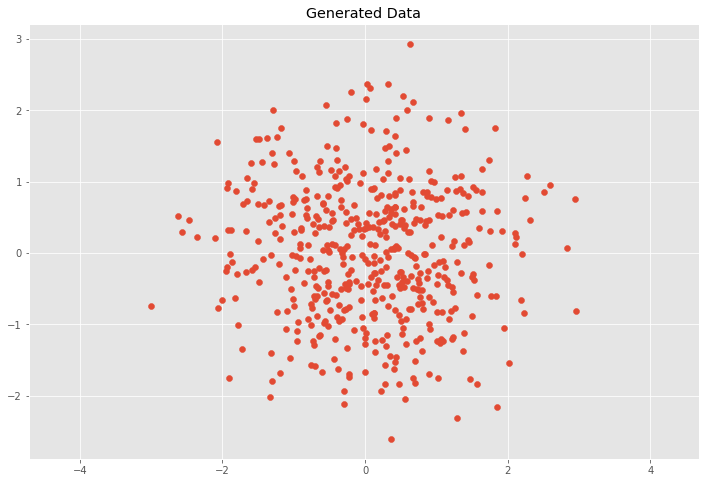
\includegraphics[scale=0.3]{uncorrelated.png}  
   \caption{Uncorrelated Variables}
\end{figure}


This case would mean that x and y are independent (or uncorrelated) and the covariance matrix C is:
$$C = \left( \begin{array}{ccc}  \sigma_x^2 & 0 \\  0 & \sigma_y^2 \end{array} \right)$$

\subsection{Linear Transformations of the Data Set}
Next, we will look at how transformations affect our data and the covariance matrix C. We will transform our data with the following scaling matrix.
$$S = \left( \begin{array}{ccc}  s_x & 0 \\  0 & s_y \end{array} \right)$$
where the transformation simply scales the x and y components by multiplying them by $s_x$ and $s_y$ respectively. What we expect is that the covariance matrix C of our transformed data set will simply be:
$$C = \left( \begin{array}{ccc}  (s_x\sigma_x)^2 & 0 \\  0 & (s_y\sigma_y)^2 \end{array} \right)$$


\begin{figure}[h!]
  \centering
    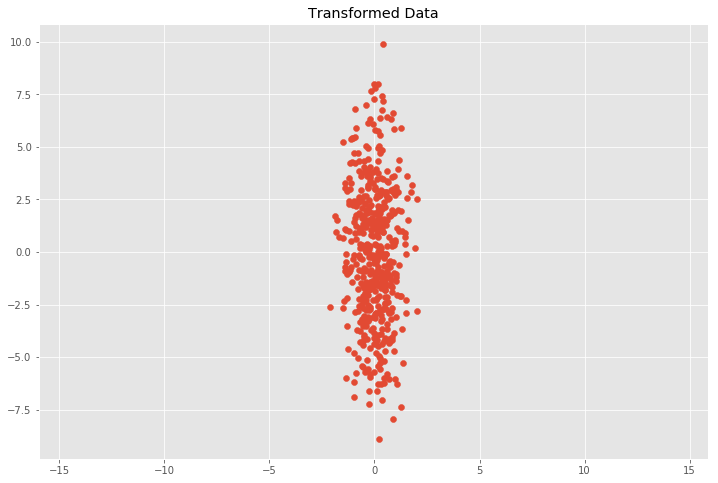
\includegraphics[scale=0.3]{uncorrelated_scaled.png}  
   \caption{Uncorrelated Scaled Variables}
\end{figure}

Now we will apply a linear transformation in the form of a transformation matrix T to the data set which will be composed of a two dimensional rotation matrix R and the previous scaling matrix S as follows: $$T = RS$$ where the rotation matrix R is given by:
$$R = \left( \begin{array}{ccc}  cos(\theta) & -sin(\theta) \\  sin(\theta) & cos(\theta) \end{array} \right)$$

where $\theta$ is the rotation angle. The transformed data is then calculated by Y=TX or Y=RSX and the covariance matrix are $$YY^T=RSX(RSX)^T=RSXX^TS^TR^T=RSCS^TR^T=R\left( \begin{array}{ccc}  (s_x\sigma_x)^2 & 0 \\  0 & (s_y\sigma_y)^2 \end{array} \right)R^T$$.

\begin{figure}[h!]
  \centering
    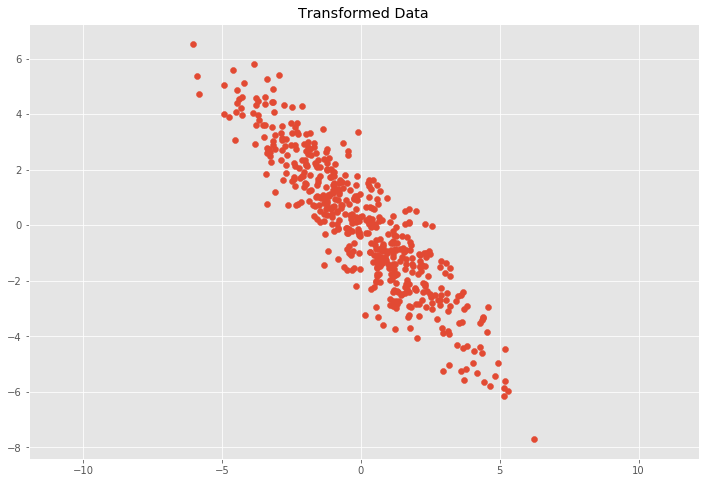
\includegraphics[scale=0.3]{correlated.png}  
   \caption{Uncorrelated Scaled Variables}
\end{figure}

As we can see now, the x,y coordinate of each variable are not uncorrelated anymore. For example, if we know that the x value of the sample is high, it is more likely that the y value are low, and vice versa. Note, that R is orthogonal, thus we got the SVD decomposition of the covariance matrix. Later in the course we are going to use some of the properties of the covariance matrix and its SVD decomposition in the context of dimensionality reduction, but for now lets take a look at simple example in order to get better understand:

\begin{exercise}
let $X^T=\left(\begin{array}{cc}
150 & 45\\
170 & 74\\
184 & 79
\end{array}\right)$ be samples of hight and weight of 3 different people where $X_{1i}$ is the hight and $X_{2i}$ is the weight of the i'th man. calculate the covariance matrix of the sample.
\end{exercise}
First of all we will make the the data centered:
We have: $\bar{x_1}=168$ and $\bar{x_2}=66$, so $$X_{centered}^{T}=\left(\begin{array}{cc}
-18 & -21\\
2 & 8\\
16 & 13
\end{array}\right)$$
and: 
$$
\frac{X_{centered}X_{centered}^{T}}{3-1}=\left(\begin{array}{cc}
292 & 301\\
301 & 337
\end{array}\right)
$$

\subsection{Normal Distribution}
We now consider specific family of distributions- the "Normal Distributions". The normal distribution is useful because of the central limit theorem. In its most general form, under some conditions, it states that averages of samples of observations of random variables independently drawn from independent distributions converge in distribution to the normal, that is, they become normally distributed when the number of observations is sufficiently large. Moreover, many results and methods (such as propagation of uncertainty and least squares parameter fitting) can be derived analytically in explicit form when the relevant variables are normally distributed. 

\begin{definition}[Normal Distribution]
random vriable x has a normal distribution with expectation $\mu$ and covariance $\Sigma$ if it has a PDF of the form:
$$f(x \mid \mu, \sigma^2) = \frac{1}{\sqrt{2\pi\sigma^2} } e^{ -\frac{(x-\mu)^2}{2\sigma^2} } $$
In this case we write: $x\sim\mathcal{N}({\mu},{\sigma^2})$

\end{definition}
\begin{definition}[Multivariate Normal Distribution]
random vector x has a multivariate normal distribution with expectation $\mu$ and covariance $\Sigma$ if it has a joint PDF of the form:
$$f_{x}\left(X\right)=\frac{1}{\sqrt{\left(2\pi\right)^{n}\left|\Sigma\right|}}\exp\left\{ -\frac{\left(x-\mu\right)^{T}\Sigma^{-1}\left(x-\mu\right)}{2}\right\} $$
In this case we write: $x\sim\mathcal{N}(\boldsymbol{\mu},\boldsymbol{\Sigma})$
\end{definition}

Observe that definition 10 is generalization of 9, i.e. when n=1 both definitions are same.
\\

In some cases we do not care about some of the variables in the distribution. for example, suppose we have joint probability function of the variables "height" and "weight" of some community, but we only interested in one of them. this lead as to the following definition:

\begin{definition}[Marginal Distribution]
Marginal distribution of a subset of a collection of random variables is the probability distribution of the variables contained in the subset. It gives the probabilities of various values of the variables in the subset without reference to the values of the other variables. It can be written as:
$$p_{X}(x)=\int_{y}p_{X,Y}(x,y)\mathrm{d}y$$
\end{definition}

\begin{exercise}[Marginal of multivariate normal distribution] 
Let $x\sim\mathcal{N}(\boldsymbol{\mu},\boldsymbol{\Sigma})$ where $\mu = (\mu_1, \mu_2), \boldsymbol{\Sigma}=\left(\begin{array}{cc}
\sigma_{1}^{2} & 0\\
0 & \sigma_{2}^{2}
\end{array}\right)$.

Find the PDF of the marginal distribution of $x_1$.
\end{exercise}

Solution:

Observe that we have:

\begin{align*}
\frac{1}{\sqrt{\left(2\pi\right)^{n}\left|\Sigma\right|}}\exp\left\{ -\frac{\left(x-\mu\right)^{T}\Sigma^{-1}\left(x-\mu\right)}{2}\right\} &= \frac{1}{\sqrt{\left(2\pi\right)^{2}\left|\left(\begin{array}{cc}
\sigma_{1}^{2} & 0\\
0 & \sigma_{2}^{2}
\end{array}\right)\right|}}\exp\left\{ -\frac{\left(x-\mu\right)^{T}\left(\begin{array}{cc}
\sigma_{1}^{-2} & 0\\
0 & \sigma_{2}^{-2}
\end{array}\right)\left(x-\mu\right)}{2}\right\}\\& 
= \frac{1}{\sqrt{\left(2\pi\right)^{2}\sigma_{1}^{2}\sigma_{2}^{2}}}\exp\left\{ -\frac{\left(x-\mu\right)^{T}\left(\begin{array}{cc}
\sigma_{1}^{-2} & 0\\
0 & \sigma_{2}^{-2}
\end{array}\right)\left(x-\mu\right)}{2}\right\} \\&
= \frac{1}{\sqrt{\left(2\pi\right)^{2}\sigma_{1}^{2}\sigma_{2}^{2}}}\exp\left\{ -\left(\frac{x_{1}-\mu_{1}}{2\sigma_{1}}\right)^{2}-\left(\frac{x_{2}-\mu_{2}}{2\sigma_{2}}\right)^{2}\right\} \\&
=	\frac{1}{\sqrt{\left(2\pi\right)\sigma_{1}^{2}}}\exp\left\{ -\left(\frac{x_{1}-\mu_{1}}{2\sigma_{1}}\right)^{2}\right\} \frac{1}{\sqrt{\left(2\pi\right)\sigma_{2}^{2}}}\exp\left\{ -\left(\frac{x_{2}-\mu_{2}}{2\sigma_{2}}\right)^{2}\right\} 
\end{align*}

Now, since: $\int_{x_2}\frac{1}{\sqrt{\left(2\pi\right)\sigma_{2}^{2}}}\exp\left\{ -\left(\frac{x_{2}-\mu_{2}}{2\sigma_{2}}\right)^{2}\right\} 
\mathrm{d}x_2=1$, we get $x_1\sim\mathcal{N}({\mu_1},{\sigma_1^2})$
\\

Curious student may ask- what if $\sigma_{1,2}\neq 0$? the answer is that we can show that the marginal distribution is also normal, but it require some more algebric transitions so we will not show it here. 

Finally we just mention that the result above identical even if we have more than 2 variables, i.e. $x_1=(x_1^1...x_1^k), x_2=(x_2^1...x_2^l), \sigma_1^2=\Sigma_1, \sigma_2^2=\Sigma_2$


\section{Probability Inequalities}
\subsection{Motivation and Background}
\footnote{This section based on lecture notes by Michal Moshkovitz and Alon Gonen} Probability inequalities is very useful in analyzing random processes. In particular, it is used to analyze machine learning algorithms. The first and the most standard result of concentration results is for
averages. It states that the average of bounded independent random variables is concentrated around its expectation. As we will see in class, in many
learning tasks, we wish to estimate the expectation of some random variable
(e.g. the generalization error of a hypothesis) using the average of independently and identically i.i.d distributed random variables (e.g. the empirical loss of the same hypothesis). The law of large numbers states that the empirical average converges to the expected value. Probability inequalities provides us a means by which we can tell how good our estimates are when the sample is finite.

For being more concrete, consider the following task. Suppose that
there is a bag containing red and blue balls. We would like to
estimate the fraction $p$ of red balls in the bag. However, we are only
allowed to sample randomly from the bag with replacement. The
straightforward strategy is to draw $n$ samples and predict
\[
\hat{p} = \frac{\# ~\text{of red balls}}{n}~.
\]
It is clear that $\E [\hat{p}] = p$. However, we might err due to the
fact that we get only limited information. Thus, we are
interested in estimation with certain additive error
$\epsilon$. Another obstacle is that since our process is random,
there is a probability that our sample doesn't represent the
distribution ``well''. Thus, we will further refine our objective. We will
be interested to guarantee with high probability that our estimator
has an additive error at most $\epsilon$. 

More generally, concentration inequalities deal with the following fundamental
question: Given an accuracy parameter $\epsilon > 0$ and a confidence
parameter $\delta \in (0,1)$, how many samples are needed to guarantee that with probability at least $1- \delta$, our estimate is within additive error of at most
$\epsilon$. The corresponding notion in supervised learning is named
\emph{probably approximately correct (PAC)
learnability}. That is, we aim at constructing a learner whose
estimations are probably (with probability at least $1-\delta$)
approximately (within additive error of at most $\epsilon$) correct.

The exact formulation of the PAC framework will be given in the
lecture. In this Tirgul, we will consider the well-known challenge of
estimating the bias of a given coin. As we shall see, this moderate
challenge hides within itself many of the ingredients of the PAC framework.

\subsection{Recap} \label{sec:recap}
We are already familiar with some concentration inequalities. We next recall Markov's and Chebyshev's inequalities and apply both inequalities to derive concentration inequalities for averages.
\begin{theorem} \textbf{Markov's inequality:} For a nonnegative random
variable $X$ (i.e. $\text{Im}(X) \subseteq \reals_{\ge 0}$) with finite mean and a positive scalar $t$,
\[
\prob [X \geq t] \leq \frac{\mathbb{E}[X]}{t}~.
\]
\end{theorem}
\begin{proof}
Let $f(x)$ be the density function of $x$. Since $X$ is non-negative, we obtain
\begin{align*}
\E[X] &= \int_{x \in \reals} f(x) x \,dx \\&
= \int_{x = 0} ^t f(x) x\, dx + \int_{x =t} ^\infty f(x) x \, dx \\&
\ge \int_{x =t} ^\infty f(x) x \,dx \\&
\ge \int_{x =t} ^\infty f(x) t \, dx\\&
= t \cdot \int_{x =t} ^\infty f(x) \,dx \\&
=t \cdot \prob[X \ge t] ~.
\end{align*}
The desired inequality is obtained by dividing both sides by $t$.
\end{proof}
By the linearity of expectation, we obtain an identical bound for averages.
\begin{corollary} \label{cor:markovAve}
Let $X$ be a nonnegative random variable with finite mean. Denote its distribution by $\cD$. Let $X_1,\ldots,X_m$ be $m$ i.i.d. copies of $X$, i.e., $X_1,\ldots,X_m$ are i.i.d. random variables which are distributed according to $\cD$. Denote their average by $\overbar{X}=\frac{1}{m} \sum_{i=1} ^m X_i$. Finally, let $t$ be a positive scalar. Then
\[
\prob [\overbar{X} \geq t] \leq \frac{\mathbb{E}[X]}{t}~.
\]
\end{corollary}
\begin{proof}
By the linearity of the expectation,
\begin{align*}
\bE [\bar{X}] &= \bE \left[\frac{1}{m} \sum_{i=1} ^m X_i \right] \\&
= \frac{1}{m} \sum_{i=1} ^m \bE[X_i] \\&
= \frac{1}{m} \sum_{i=1} ^m \bE[X] \\&
= \bE[X]~.
\end{align*}
Applying Markov's inequality, we obtain the desired bound.
\end{proof}

Applying Markov inequality to the random variable $(X-\E[X])^2$, we obtain Chebyshev's inequality.
\begin{theorem} \textbf{Chebyshev's inequality:} For a random variable
  $X$ with finite mean and variance, and for every $t  > 0$,
\[
\prob[|X-\E [X]| \geq t] \leq \frac{Var[X]}{t^2}.
\]
\end{theorem}
\begin{proof}
Simply observe that $\prob[|X-\E [X]| \geq t] = \prob[(X-\E [X])^2 \geq t^2]$ and apply Markov's inequality.
\end{proof}
Unlike the expectation, the variance of the average of i.i.d. random variables is not equal to the variance of the original random variable. Concretely, for a random variable $X$ and $m$ i.i.d. copies of $X$, denoted $X_1,\ldots, X_m$, we have
\begin{align} \label{eq:varAve}
\rV \left[\frac{1}{m} \sum_{i=1} ^m X_i \right] &= \frac{1}{m^2} \rV \left[\sum_{i=1} ^m X_i \right] \notag \\&
= \frac{1}{m^2} \sum_{i=1} ^m \rV [X_i] \notag \\&
= \frac{1}{m^2} \sum_{i=1} ^m \rV [X] \notag \\&
= \frac{1}{m} \rV[X]~.
\end{align}
In particular, the variance of the average tends to zero when $m$ tends to infinity. This leads to a much better concentration inequality.
\begin{corollary} \label{cor:chebysevAve}
Let $X$ be a nonnegative random variable with finite variance and let $X_1,\ldots,X_m$ be $m$ i.i.d. copies of $X$. Denote their average by $\overbar{X}=\frac{1}{m} \sum_{i=1} ^m X_i$. Finally, let $t$ be a positive scalar. Then
\[
\prob [|\overbar{X}-\E [\overbar{X}]| \geq t] = \prob [|\overbar{X}-\E [X]| \geq t] \leq \frac{\rV[X]}{mt^2}~.
\]
\end{corollary}

For a positive integer $k$, the $k$-th moment of a random variable $X$ is defined by $\bE[X^k]$. As we just saw, Markov's inequality exploits only information about the first moment, while Chebyshev's inequality exploits both the first and the second moments. Comparing the bounds in \corref{cor:markovAve} and \corref{cor:chebysevAve}, we see that using both the first and the second moments, we obtain better concentration inequalities than using only the first. We shall see soon that more generally, the more moments we use, the better the bounds that we get.


\subsection{Coin Prediction}  \label{sec:basicConcentration}
Let us formulate the problem of estimating the bias of a
coin (in short, coin prediction)\footnote{We take this opportunity to recall some basic notions from probability theory}. Formally, a coin is a Bernoulli random variable $Z$ with a bias $p$ ($p$ is the probability to obtain a ``head''). %The probability space which is associated with $Z$ is the triplet $(\Omega ,\prob )$, where the sample space $\Omega$ equals $\{H,T\}$,  $$\prod\{1\}]=p~,~\cD[\{0\}]=1-p~. $$Once we defined $\cD(\{1\})$ and $\cD(\{0\})$, the values of $\cD$ on other events are determined by combining the fact that $\cD$ is additive (for disjoints subsets $E,F \in \cF$, we have $\cD(E \cup F)=\cD(E) + \cD(F)$) with the fact that $\cD(\Omega)=1$.
The random variable $Z$ is simply a function from $\Omega$ to
$\{0,1\}$. Let $Z_1,
\ldots, Z_m$ be a sequence of independent and identically distributed
(i.i.d.) random variables according to the distribution $\cD_Z$ (that
is, each of the $Z_i$ has the same distribution as $Z$, and all of the
$Z_i$ are mutually independent). Denote the random sequence  (a.k.a. sample)
$(Z_1,\ldots, Z_m)$ by $S$. The distribution which is associated with $S$ is denoted by $\cD_Z ^m$ (or simply by $\cD^m$).

The input of a \emph{learning algorithm} $A$ for the task of coin prediction
consists of a random sequence $S$ which is drawn according to
$\cD^m$. Based on this input, the algorithm has to predict the value
of $p$. We denote this prediction by $A(S)$ or simply by
$\hat{p}$. Clearly, the drawn sequence can not fully describe the
distribution. Hence, we introduce an \emph{accuracy} parameter $\epsilon>0$
and allow $\hat{p}$ to deviate from $p$ by at most $\epsilon$. Furthermore, there is always a chance that the drawn sequence would be highly non-representative, so it is impossible to obtain a guarantee that holds with absolute certainty. Hence, we introduce a
\emph{confidence} parameter $\delta>0$, and allow that
the event $B:=\{s : |\hat{p}-p|>\epsilon\}$ occur with probability at
most $\delta$. More formally:
\begin{definition}  \label{def:sampleCoin}
A learning algorithm $A$ for the task of (batch) coin prediction is a function
from $\bigcup_{m=1} ^\infty \{0,1\}^m$ to $[0,1]$ which satisfies the following
property: There exists a function $m_A:
(0,1)^2 \rightarrow \bN$, such that for every $\epsilon,\delta
\in (0,1)$ and every distribution $\cD$ that corresponds to some
bias $p \in [0,1]$, when running the algorithm on $m \ge m_A(\epsilon,\delta)$
i.i.d. examples generated according to $\cD^m$,
the algorithm returns a prediction $\hat{p}$ such that with
probability at least $1-\delta$,
\[
|p-\hat{p}| \le \epsilon~.
\]
The minimal function\footnote{That is, the function that returns the minimal integer for every $\epsilon,\delta$ such that the above requirement holds.} among the functions that satisfy the above is denoted by $m_A(\epsilon,\delta)$, and named the \emph{sample complexity} of the algorithm $A$. The sample complexity of coin prediction, denoted by $m(\cdot,\cdot)$, is the minimal function that satisfies the above (in other words, $m(\cdot, \cdot)$ is the sample complexity of the optimal algorithm for coin prediction).
\end{definition}
%The term `approximately' in PAC stems from the fact that we only require that $\hat{p}$ approximates $p$ to an accuracy $\epsilon$. The term `probably' in PAC comes from the fact that we are satisfied whenever $\hat{p}$ satisfies the accuracy requirements with probability at least$1-\delta$.

Given an i.i.d. random sample $S=(z_1, \ldots, z_m)$, a reasonable
estimate of $p$ is the empirical proportion of heads (ones), namely
$\hat{p}=\frac{1}{m} \sum_{i=1} ^m z_m$. The first basic property of
this average is that its expected value equals $p$. This follows by
the linearity of expectation as follows:
\[
\bE \left [\frac{1}{m} \sum_{i=1} ^m Z_i \right] = \frac{1}{m} \sum_{i=1} ^m
\bE[Z_i] = \frac{1}{m} \cdot m \cdot p = p~.
\]
We say in this case that $\hat{p}$ forms an \emph{unbiased estimate}
of $p$. What can we say about the quality of $\hat{p}$ as an estimate
of $p$? In other words, how tightly $\hat{p}$ is concentrated around
its expectation? To answer this question, we can use concentration inequalities.\\

\noindent \textbf{First attempt: Markov's inequality: }\\
There are two problems with applying Markov's inequality for our purpose. First, while we are interested in an upper bound on the probability of the event $|\hat{p}-p| > \epsilon$, a direct application of Markov's inequality only gives us a bound on one-side error, namely, we can obtain a bound on the probability that $\hat{p} - p > \epsilon$. However, as we shall see in the next Targil, this problem is merely technical and can be easily circumvented. The main problem is that the bound we get are very weak; In particular, as we noted in \corref{cor:markovAve}, since we only exploit information about the first moment, the obtained bound is uniform over all possible values of $m$. In particular, it does not tend to $0$ as $m$ tends to infinity.\\

\noindent \textbf{Second attempt: Chebyshev's inequality: }
The variance of a Bernoulli random variable is $p(1-p) \le 1/4$. Applying \corref{cor:chebysevAve}, we obtain that 
\[
\cD^m [|\hat{p}-p| > \epsilon] \le \frac{1}{4m \epsilon ^2}~.
\]  
We conclude the following.
% \begin{theorem}  \label{thm:basicConcentration}
% Let $A$ be an algorithm for coin prediction which given an access to an i.i.d. random sequence $S$ of size $m$, predicts with $\hat{p}$ being the
% empirical proportion of heads. Then, for every bias $p \in
% [0,1]$, and every $\epsilon \in (0,1)$, the following assertions hold:
% \begin{enumerate}
% \item
% \textbf{(The weak law of large numbers): }The average $\hat{p}$ \emph{converges in probability} to its
% expected value $p$. Formally,
% \[
% \lim_{m \rightarrow \infty} \cD^m \left [|\hat{p}-p|>\epsilon \right]=0.
% \]
% \item
% \textbf{(The strong law of large numbers): }The average $\hat{p}$
% \emph{converges almost surely} to its expected value $p$. Formally,
% \[
% \cD^\bN \left [ \lim_{m \rightarrow \infty} \hat{p}=p \right]=1.
% \]
% \item
% \textbf{(Marlov's inequality}
% \item
%\textbf{(Chebyshev's inequality): }
% \[
% \cD^m [|\hat{p}-p|>\epsilon ] \le \frac{1}{4m \epsilon^2}~.
% \]
% \end{theorem}

% \begin{proof}
% \end{proof}

\begin{corollary}  \label{cor:basicConcentration}
The sample complexity of coin prediction is bounded above by
$m(\epsilon,\delta) \le \left \lceil \frac{1}{4\epsilon^2} \cdot
  \frac{1}{\delta} \right \rceil$.
\end{corollary}

A natural question which arises is whether the obtained bound is optimal (tight). There is a good reason to suspect that this bound is not optimal; When we applied Markov's inequality, we only relied on the non-negativity of our random variables. We did not exploit the fact that they are bounded (between $0$ and $1$) and independent. Indeed, in the next section we prove a much better bound\footnote{Which is tight but we will not prove the optimality}. For this end, we will introduce Hoeffding's inequality for the average of independent and bounded random variables. This inequality will give us exponential (instead of polynomial!) convergence. 
\subsubsection{Hoeffding's Inequality}
\begin{theorem} (Hoeffding's inequality)
Let $X_1, \ldots X_m$ be independent and bounded random variables with $a_i \leq X_i \leq b_i$. Let $\bar{X} = \frac{1}{m} \sum_{i=1} ^m X_i$. Then,
\[
\prob [ |\bar{X} - \E[\bar{X}]| \geq \epsilon ] \leq 2 \exp(-2m^2 \epsilon^2 / \sum _{i =1} ^m (b_i-a_i)^2)~.
\]
\end{theorem}
\begin{corollary}
Let $X_1, \ldots X_m$ be a sequence of i.i.d. (independent and identically distributed) and bounded with $a \leq X_i \leq b$. Let $\bar{X} = \frac{1}{m} \sum_{i=1} ^n X_i$ and let $\mu = \E[X_i]$. Then,
\[
\prob [|\bar{X} - \mu| \geq \epsilon] \leq 2 \exp(-2 m \epsilon^2 / (b-a)^2) 
\]
\end{corollary}

\subsubsection{Coin Prediction Revisited}
Lets apply Hoeffding's inequality for the case of coin prediction which was discussed above. For a sample of size $m$, we obtain 
\[
\cD^m [|\hat{p}-p|>\epsilon ]\leq  2 \exp(-2 m \epsilon ^2)~.
\]
Indeed, we achieve an exponential improvement (in terms of $\delta$).  
\begin{corollary}  \label{cor:basicConcentration}
The sample complexity of coin prediction is bounded above by
$m(\epsilon,\delta) \le \left \lceil \frac{1}{2\epsilon^2} \cdot
  \log(\frac{2}{\delta}) \right \rceil$.
\end{corollary}

\subsubsection{Better Rates for Unfair Coins}
The most appealing property of the bound in \corref{cor:basicConcentration} is that it is uniform over all possible values of the bias $p$. This robustness property comes with a
price: As our intuition tells us, a coin with a bias $p$ close to $0$
(or $1$) is much easier to estimate than a coin with bias close to
$1/2$. We now consider the extreme case
in which $\hat{p}=0$, i.e., there are no heads in the
sample. \corref{cor:basicConcentration} guarantees that the following
algorithm is a learning algorithm for coin prediction: Given as
an input a sample of size $m=\lceil \frac{1}{2\epsilon^2} \cdot
  \log(\frac{2}{\delta}) \rceil$, predict with the fraction of heads in
the sample. In particular, if there are no heads in the sample, predict with $\hat{p}=0$. We next improve this result. We start with the following lemma.
\begin{lemma}  \label{lem:realizableCoin}
Let $\epsilon, \delta \in (0,1)$. If a coin has a bias $p>\epsilon$,
the probability of getting no heads in $m$ flips (i.e., $\hat{p}=0$)
is at most $\exp(-\epsilon m)$. 
\end{lemma}
\begin{proof} 
Assume that $p>\epsilon$. The probability of obtaining no heads is
given by $(1-p)^m$. Using the inequality $1-x \le \exp(-x)$, which
holds for every $x \in \reals$, we obtain that this probability is at
most
\[
\exp(-pm) \le \exp(-\epsilon m)~.
\]
\end{proof}
Let us discuss the implications of
\lemref{lem:realizableCoin}. Consider the following learning rule:
Observe a sample of size $\left \lceil \frac{\log(2/\delta)}{\epsilon}
\right \rceil$. If there are no heads, return $\hat{p}=0$. Otherwise, observe an 
additional sample of size $\lceil \frac{1}{2\epsilon^2} \cdot
  \log(\frac{4}{\delta}) \rceil - \left \lceil \frac{\log(2/\delta)}{\epsilon}
\right \rceil$, and predict with the fraction of heads in the whole
sequence. Denote this algorithm by $A$. We will soon prove that $A$ is a learning algorithm for the task of coin prediction. Before that, note that in terms of sample complexity we do not obtain any improvement; In the worst case ($\hat{p} \neq 0$) we need (asymptotically) the same amount of samples. However, if $\hat{p} = 0$, we do obtain a dramatic improvement; The required amount of examples in this case scale with $1/\epsilon$ which is smaller that $1/\epsilon^2$ since $\epsilon \in (0,1)$\footnote{This gap might be very large. For example, if we require an accuracy of $\epsilon=0.001$, we have $1/\epsilon=10^3$, while $1/\epsilon^2 = 10^6$}.

We next show that $A$ is a learning algorithm for coin prediction, we need to recall the following important lemma. 

\begin{theorem}
The algorithm A is a learning algorithm for coin prediction.
\end{theorem}
\begin{proof}
Let $\epsilon,\delta \in (0,1)$. Let $p$ be a bias, and let $\cD$ be the corresponding distribution. If $p> \epsilon$, let $E$ be the event
consisting of all sequences of size $\left \lceil \frac{\log(2/\delta)}{\epsilon}
\right \rceil$ which contain no heads. If $p \le \epsilon$, let
$E=\emptyset$. Let $F$ be the event consisting of all sequences of size $\lceil \frac{1}{2\epsilon^2} \cdot
  \log(\frac{4}{\delta})  \rceil$ for which $|\hat{p}-p|>\epsilon$. Note
that the probability of both events is bounded above by
$\delta/2$. Also, note that if the event $E \cup F$ does not occur, the
output $\hat{p}$ of $A$ satisfies $|\hat{p}-p| \le \epsilon$. We apply the
union bound to complete the proof. 
\end{proof}

\end{document}